\section{Ergänzende Datenauswertungen}
\label{appendix}

\begin{figure}[!htb]
    \centering
    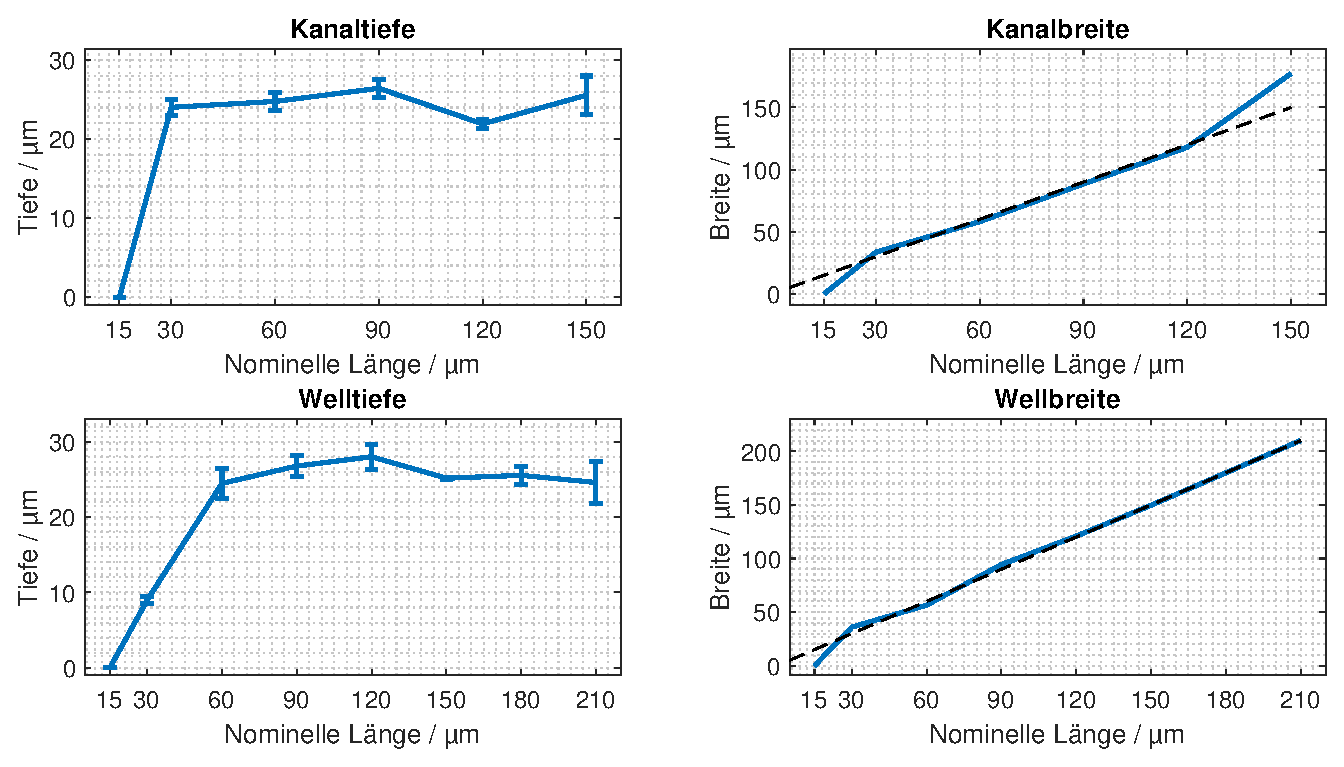
\includegraphics[width=\linewidth]{plot/25um_SL_ResolutionV1.eps}
    \caption{Profilometrie des \SI{25}{\micro\meter}-Einzellayers aus MPC.}
    \label{fig:MPC_25um}
\end{figure}


\begin{figure}[!htb]
    \centering
    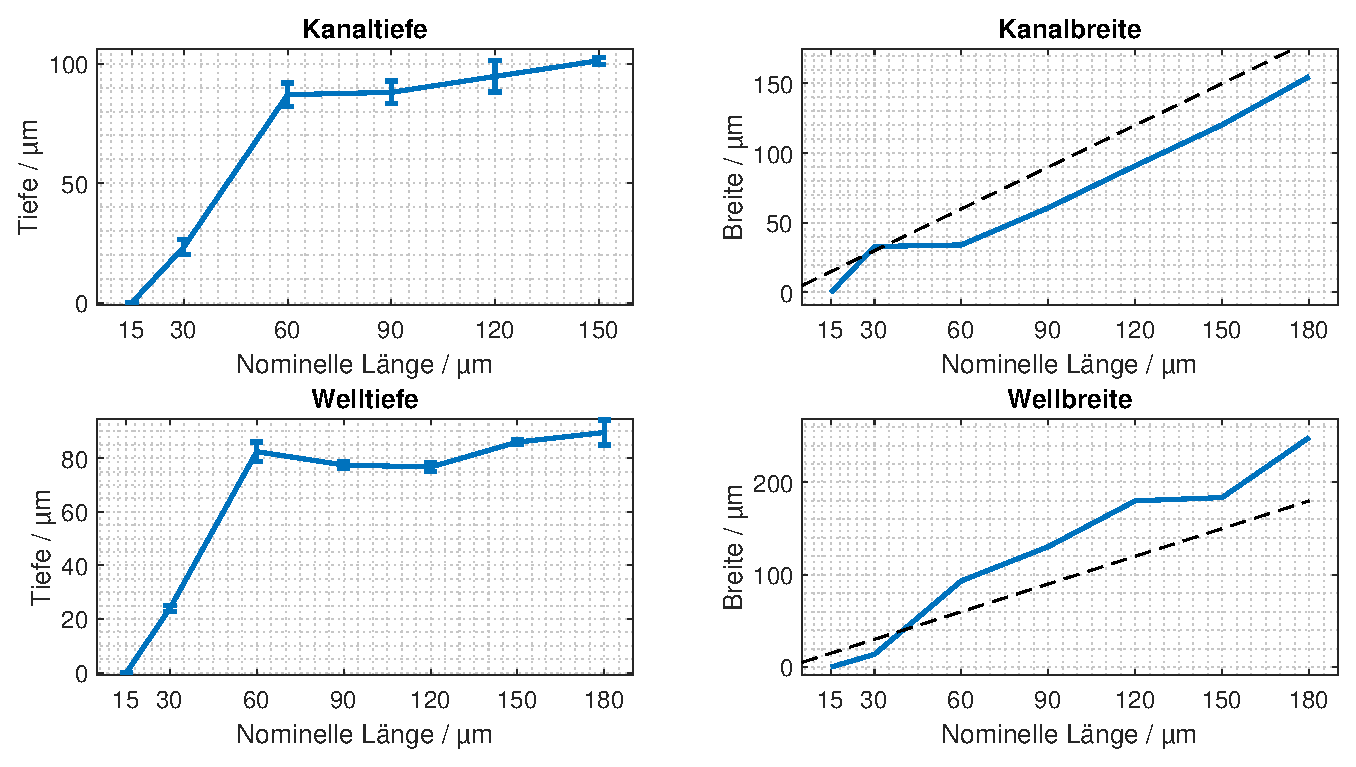
\includegraphics[width=\linewidth]{plot/100um_SL_ResolutionV1.eps}
    \caption{Profilometrie des \SI{100}{\micro\meter}-Einzellayers aus MPC.}
    \label{fig:MPC_100um}
\end{figure}

\begin{figure}[!htb]
    \centering
    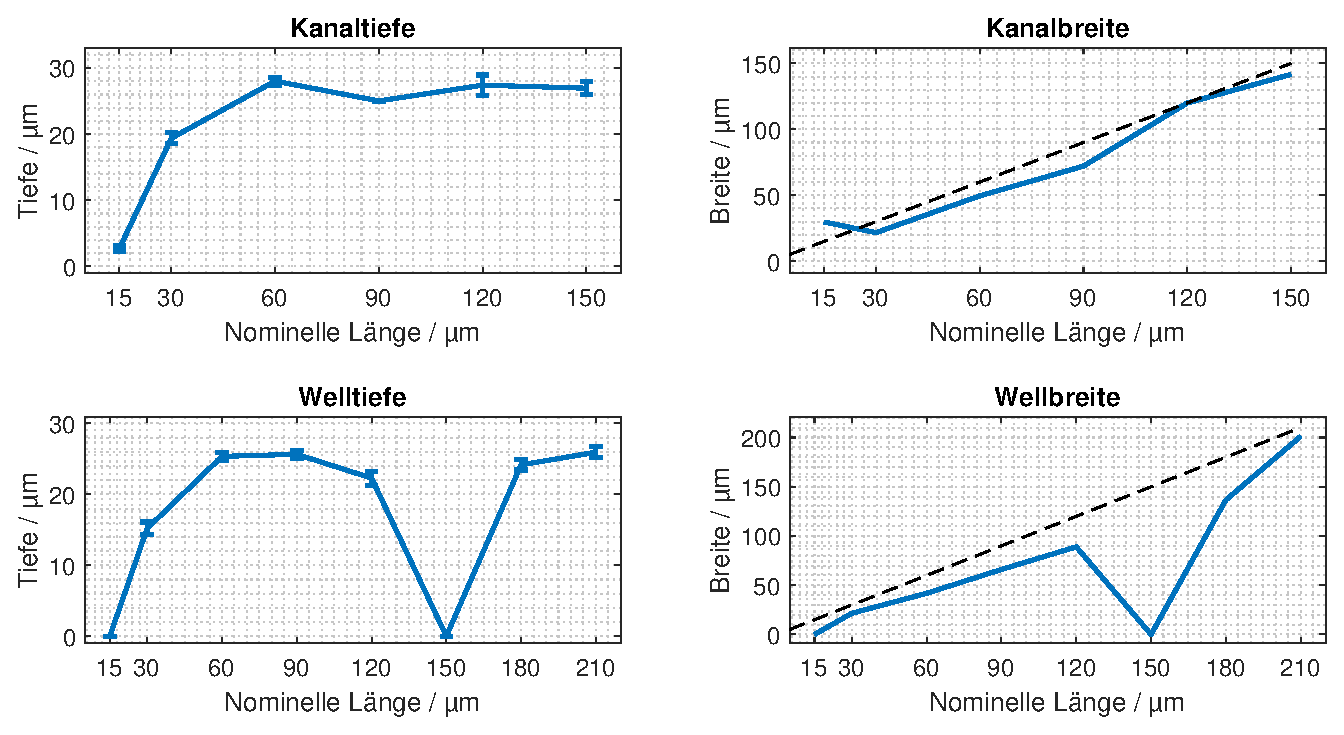
\includegraphics[width=\linewidth]{plot/PEGDA_25um_SL_ResolutionV1.eps}
    \caption{Profilometrie des \SI{25}{\micro\meter}-Einzellayers aus PEGDA.}
    \label{fig:PEGDA_25um}
\end{figure}

\begin{figure}[!htb]
    \centering
    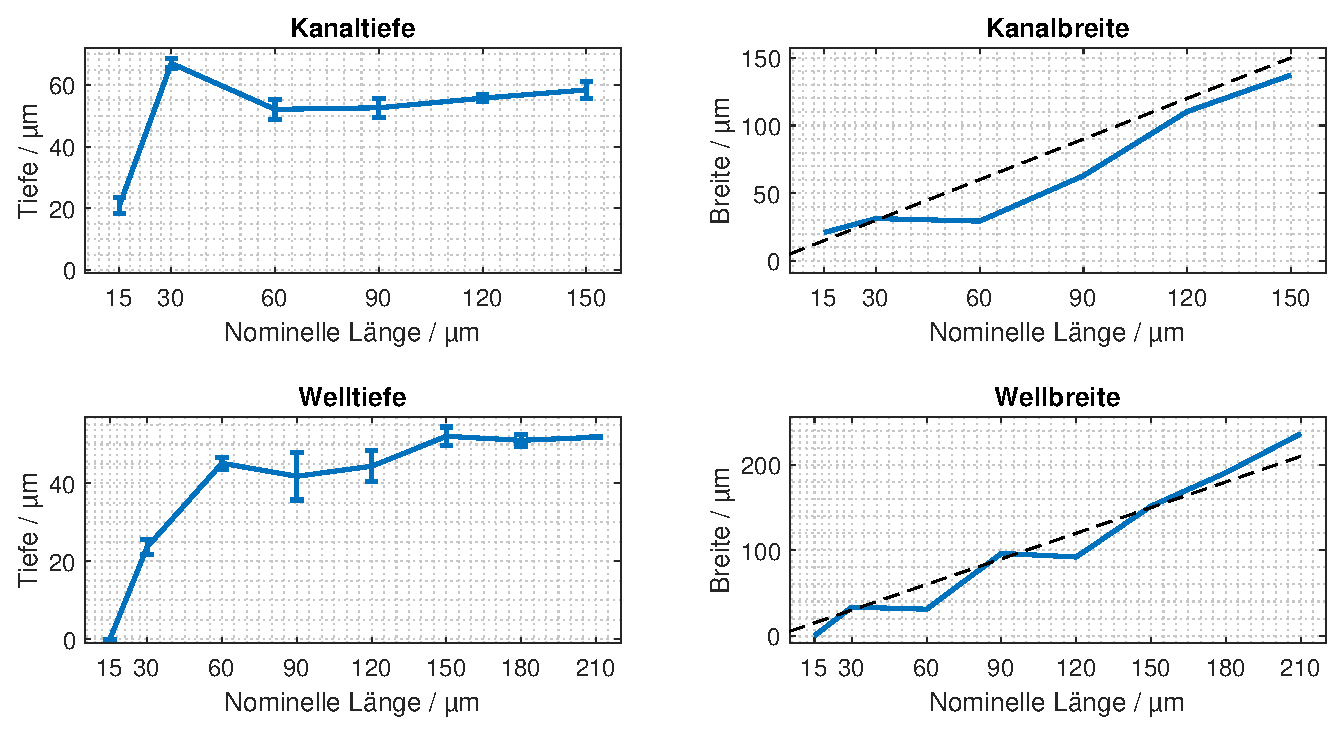
\includegraphics[width=\linewidth]{plot/PEGDA_50um_SL_ResolutionV1.eps}
    \caption{Profilometrie des \SI{50}{\micro\meter}-Einzellayers aus PEGDA.}
    \label{fig:PEGDA_50um}
\end{figure}